%%%%%%%%%%%%%%%%%%%%%%%%%%%%%%%%%%%%%%%%%%%%%%%%%%%%%%%%%%%%%%%%%%%%%%%% 
%%%%%%%%%%%%%%%%%%%%%%%%%%%%%%%%%%%%%%%%%%%%%%%%%%%%%%%%%%%%%%%%%%%%%%%% 
\begin{frame}[fragile=singleslide]
  \frametitle{Kokkos - cmake integration (1)}

  \begin{itemize}
  \item Why Cmake ?
    \begin{itemize}
    \item cmake is supported by kokkos
    \item easy to integrate and configure (versus e.g. old autotools, versus regular Makefile): need to handle the architecture flags combinatorics
    \end{itemize}
  \item User application top-level cmake can be as small as 7 lines
    {\small
      \begin{minted}{cmake}
        cmake_minimum_required(VERSION 3.1)
        project(myproject CXX)
        
        # C++11 is for Kokkos
        set(CMAKE_CXX_STANDARD 11)
        set(CMAKE_CXX_EXTENSIONS OFF)
        
        # first buid kokkos
        add_subdirectory(external/kokkos)
        
        # pass Kokkos include directories to our target application
        include_directories(${Kokkos_INCLUDE_DIRS_RET})
        
        # build the user sources
        add_subdirectory(src)
      \end{minted}
      }
  \end{itemize}
  
\end{frame}

%%%%%%%%%%%%%%%%%%%%%%%%%%%%%%%%%%%%%%%%%%%%%%%%%%%%%%%%%%%%%%%%%%%%%%%% 
%%%%%%%%%%%%%%%%%%%%%%%%%%%%%%%%%%%%%%%%%%%%%%%%%%%%%%%%%%%%%%%%%%%%%%%% 
\begin{frame}[fragile=singleslide]
  \frametitle{Kokkos - cmake integration (2)}

  {\large List of important kokkos-related {\bf cmake variables}}
  \begin{itemize}
  \item \textcolor{magenta}{\texttt{KOKKOS\_ENABLE\_OPENMP}}, \textcolor{magenta}{\texttt{KOKKOS\_ENABLE\_CUDA}},... $\Rightarrow$ which execution space are enabled (multiple possible)
  \item \textcolor{magenta}{\texttt{KOKKOS\_ARCH}} (bold values are relevant for \texttt{ouessant}), will trigger relevant arch flags
    \begin{tabular}{ll}
      \# Intel:    & KNC,KNL,SNB,HSW,BDW,SKX\\
    \# NVIDIA:   & Kepler,Kepler30,Kepler32,Kepler35,\textcolor{red}{\bf Kepler37},Maxwell,\\
      & Maxwell50,Maxwell52,Maxwell53,\textcolor{red}{\bf Pascal60},Pascal61,\\
      & Volta70,Volta72\\
    \# ARM:      &ARMv80,ARMv81,ARMv8-ThunderX,ARMv8-TX2\\
    \# IBM:      &BGQ,Power7,\textcolor{red}{\bf Power8},Power9\\
    \# AMD-GPUS: &Kaveri,Carrizo,Fiji,Vega\\
    \# AMD-CPUS: &AMDAVX,Ryzen,Epyc\\
    \end{tabular}
    % # possible values:
    % # Intel:    KNC,KNL,SNB,HSW,BDW,SKX
    % # NVIDIA:   Kepler,Kepler30,Kepler32,Kepler35,Kepler37,Maxwell,
    %             Maxwell50,Maxwell52,Maxwell53,Pascal60,Pascal61,
    %             Volta70,Volta72
    % # ARM:      ARMv80,ARMv81,ARMv8-ThunderX,ARMv8-TX2
    % # IBM:      BGQ,Power7,Power8,Power9
    % # AMD-GPUS: Kaveri,Carrizo,Fiji,Vega
    % # AMD-CPUS: AMDAVX,Ryzen,Epyc
  \end{itemize}

\end{frame}

%%%%%%%%%%%%%%%%%%%%%%%%%%%%%%%%%%%%%%%%%%%%%%%%%%%%%%%%%%%%%%%%%%%%%%%% 
%%%%%%%%%%%%%%%%%%%%%%%%%%%%%%%%%%%%%%%%%%%%%%%%%%%%%%%%%%%%%%%%%%%%%%%% 
\begin{frame}[fragile=singleslide]
  \frametitle{Kokkos - cmake integration (3)}

  \begin{itemize}
  \item curse gui interface: \texttt{ccmake}
    \begin{center}
      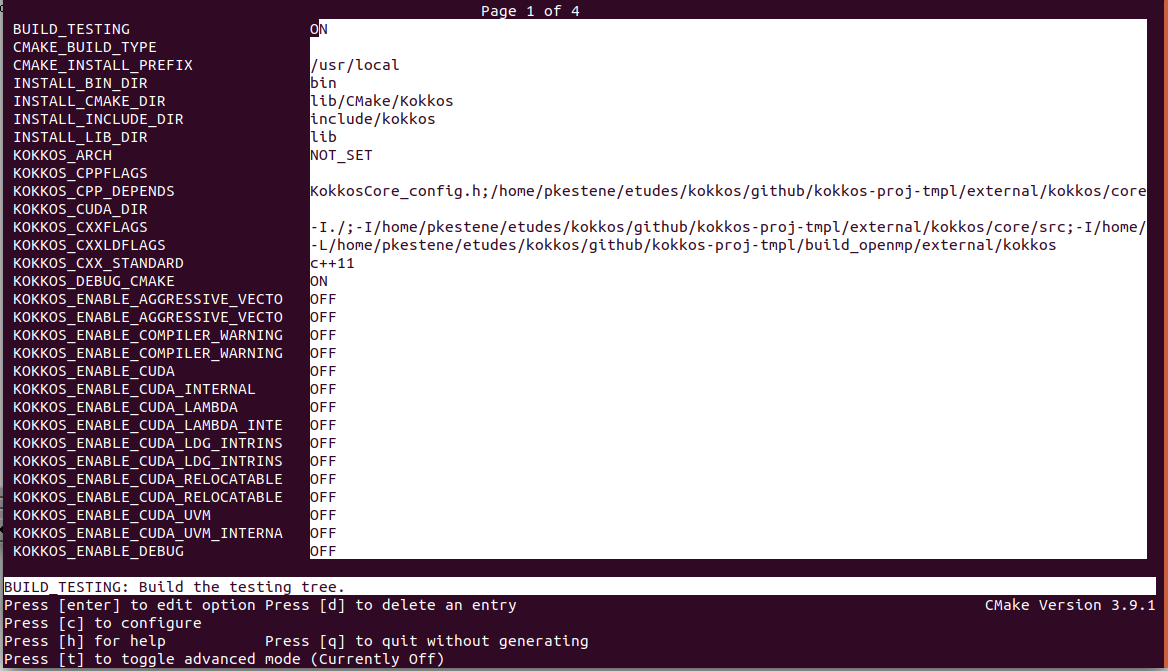
\includegraphics[width=7cm]{images/ccmake_kokkos}
    \end{center}
  \item command line interface : \texttt{cmake}
    \texttt{mkdir build\_openmp; cd build\_openmp; ccmake -DKOKKOS\_ENABLE\_OEPNMP ..}
  \item How to build ? for OpenMP / CUDA ?
  \end{itemize}

\end{frame}
  
%%%%%%%%%%%%%%%%%%%%%%%%%%%%%%%%%%%%%%%%%%%%%%%%%%%%%%%%%%%%%%%%%%%%%%%%
%%%%%%%%%%%%%%%%%%%%%%%%%%%%%%%%%%%%%%%%%%%%%%%%%%%%%%%%%%%%%%%%%%%%%%%% 
\begin{frame}[fragile=singleslide]
  \frametitle{Hands-On 3a}

  {\large \bf Activity: Use the template cmake / kokkos project}

  \begin{itemize}
  \item \textcolor{red}{\bf Clone the template project:}
  \end{itemize}
  {\small
    \begin{minted}{shell}
      git clone --recursive https://github.com/pkestene/kokkos-proj-tmpl.git
    \end{minted}
  }
  %
  \begin{itemize}
  \item \textcolor{blue}{Build the sample application (saxpy)}: use \texttt{ccmake} interface to setup the Kokkos OpenMP target; then try to setup the CUDA target (for arch Kepler37)
  \end{itemize}
  {\small
    \begin{minted}{shell}
      mkdir build_openmp; cd build_openmp; ccmake ..
      # set KOKKOS_ENABLE_OPENMP to ON
      make
    \end{minted}
  }
  % 
  \begin{itemize}
  \item \textcolor{blue}{Build the sample application (saxpy)}: repeat as above to setup the Kokkos CUDA target (for arch Kepler37)
  \end{itemize}
  %
  {\small
    \begin{minted}{shell}
      # don't forget to set environment variable CXX
      # export CXX="full path to nvcc_wrapper"
      mkdir build_cuda_kepler37; cd build_openmp; ccmake ..
      # set KOKKOS_ENABLE_CUDA to ON; set KOKKOS_ARCH
      make
    \end{minted}
  }
  %
  \begin{itemize}
  \item \textcolor{blue}{Try to add another executable}; e.g. copy of the tutorial \texttt{01\_hello\_world}
  \end{itemize}

\end{frame}

